\documentclass[aspectratio=169, 10pt]{beamer}

\usetheme{Madrid}
\usecolortheme{seahorse}
\setbeamertemplate{navigation symbols}{}
\setbeamertemplate{footline}[frame number]
\setbeamertemplate{itemize items}[circle]
\setbeamersize{text margin left=5mm, text margin right=5mm}

\usepackage{amsmath,amssymb}
\usepackage{booktabs}
\usepackage{graphicx}
\usepackage{xcolor}
\usepackage{tikz}
\usetikzlibrary{arrows.meta, positioning, shapes.geometric, fit, calc}
\usepackage{colortbl}
\usepackage{adjustbox}

% Custom colors
\definecolor{stageblue}{RGB}{41,98,255}
\definecolor{paramred}{RGB}{200,50,50}
\definecolor{goodgreen}{RGB}{34,139,34}
\definecolor{warnorg}{RGB}{200,120,0}
\definecolor{lightgray}{RGB}{240,240,240}
\definecolor{highlight}{RGB}{255,255,180}

\newcommand{\param}[1]{\textcolor{paramred}{\texttt{#1}}}
\newcommand{\stage}[1]{\textcolor{stageblue}{\textbf{Stage #1}}}
\newcommand{\good}[1]{\textcolor{goodgreen}{#1}}
\newcommand{\warn}[1]{\textcolor{warnorg}{#1}}

\title[SCA-CEM Hyperparameter Sweep]{\textbf{SlotCrossAttention-CEM}\\Hyperparameter Sweep for MIA Defense\\in Split Learning on FaceScrub}
\author{Group Meeting Presentation}
\date{March 2026}

\begin{document}

% ============================================================================
\begin{frame}
\titlepage
\end{frame}

% ============================================================================
\begin{frame}{Overview: What Are We Doing?}

\begin{block}{Goal}
Beat the original paper's SOTA defense against Model Inversion Attacks (MIA)\\
on FaceScrub (530 identities). \textbf{Baseline Inference SSIM $\approx$ 0.532} (lower = better privacy).
\end{block}

\vspace{0.3cm}

\begin{columns}[T]
\begin{column}{0.48\textwidth}
\textbf{Our Innovation: SCA\_new}
\begin{itemize}
    \item Replace hard KMeans clustering with \textbf{differentiable Slot Attention}
    \item End-to-end trainable CEM defense
    \item No per-epoch full-dataset re-clustering
\end{itemize}
\end{column}
\begin{column}{0.48\textwidth}
\textbf{Experiment: \texttt{run3.sh}}
\begin{itemize}
    \item \textbf{20 experiments}, 6 groups (A--F)
    \item Systematically sweep key hyperparameters
    \item Each experiment: 300--360 epochs training + 50 epochs attack evaluation
\end{itemize}
\end{column}
\end{columns}

\end{frame}

% ============================================================================
\begin{frame}{Architecture Pipeline: 8 Stages}

\begin{center}
\begin{tikzpicture}[
    node distance=0.1cm and 0.25cm,
    stage/.style={rectangle, rounded corners, draw=#1, fill=#1!10, text width=3cm, minimum height=0.7cm, align=center, font=\scriptsize},
    arrow/.style={-{Stealth[length=2.5mm]}, thick, draw=gray!70},
    plabel/.style={font=\tiny\ttfamily, text=paramred},
]
% Row 1
\node[stage=blue!70] (s1) {\textbf{Stage 1}\\Encoder $f(x)\!\to\!z$};
\node[stage=teal!70, right=0.4cm of s1] (s2) {\textbf{Stage 2}\\Noise $z_n\!=\!z\!+\!\mathcal{N}$};
\node[stage=violet!70, right=0.4cm of s2] (s3) {\textbf{Stage 3}\\Slot Attention};
\node[stage=purple!70, right=0.4cm of s3] (s4) {\textbf{Stage 4}\\Cross Attention};

% Row 2
\node[stage=red!60, below=0.5cm of s1] (s5) {\textbf{Stage 5}\\Var.\ Prediction};
\node[stage=orange!70, right=0.4cm of s5] (s6) {\textbf{Stage 6}\\CEM Loss};
\node[stage=green!60!black, right=0.4cm of s6] (s7) {\textbf{Stage 7}\\CE Loss};
\node[stage=brown!70, right=0.4cm of s7] (s8) {\textbf{Stage 8}\\Double Backward};

% Arrows
\draw[arrow] (s1) -- (s2);
\draw[arrow] (s2) -- (s3);
\draw[arrow] (s3) -- (s4);
\draw[arrow] (s4.south) -- ++(0,-0.1) -| (s5.north);
\draw[arrow] (s5) -- (s6);
\draw[arrow] (s2.south) -- ++(0,-0.08) -| (s7.north);
\draw[arrow] (s6) -- ++(0,-0.35) -| (s8.south);
\draw[arrow] (s7) -- (s8);

% Parameter labels
\node[plabel, below=0.01cm of s2] {noise};
\node[plabel, below=0.01cm of s3] {slots, iters};
\node[plabel, below=0.01cm of s4] {heads};
\node[plabel, above=0.01cm of s6] {var\_thr, loss\_scale};
\node[plabel, above=0.01cm of s8] {lambd};

\end{tikzpicture}
\end{center}

\vspace{0.15cm}
\small
\textbf{Cross-stage controls:}
\param{warmup} $\to$ gates Stages 3--6 (skipped during warmup) \quad
\param{epochs} $\to$ total training length

\end{frame}

% ============================================================================
\begin{frame}{Stage 1: Encoder $f(x) \to z$ \quad\small[Fixed across all experiments]}

\begin{columns}[T]
\begin{column}{0.55\textwidth}
\textbf{Architecture: VGG11-BN-SGM}
\begin{itemize}
    \item VGG11 backbone with BatchNorm
    \item Split at \texttt{cutlayer=4}
    \item Bottleneck: $\text{Conv} \to 8$ channels (\texttt{noRELU\_C8S1})
    \item \textbf{LCALayer}: Locally Competitive Algorithm for sparse coding
    \item \textbf{Sigmoid} activation (not ReLU)
\end{itemize}

\vspace{0.3cm}
\textbf{No parameters changed here.}\\
All 20 experiments use the identical encoder architecture.
\end{column}
\begin{column}{0.42\textwidth}
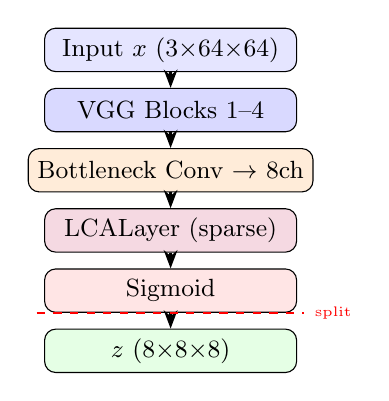
\begin{tikzpicture}[
    block/.style={rectangle, draw, rounded corners, minimum width=3.2cm, minimum height=0.55cm, align=center, font=\small},
    arr/.style={-{Stealth}, thick}
]
\node[block, fill=blue!10] (inp) {Input $x$ (3$\times$64$\times$64)};
\node[block, fill=blue!15, below=0.2cm of inp] (vgg) {VGG Blocks 1--4};
\node[block, fill=orange!15, below=0.2cm of vgg] (bn) {Bottleneck Conv $\to$ 8ch};
\node[block, fill=purple!15, below=0.2cm of bn] (lca) {LCALayer (sparse)};
\node[block, fill=red!10, below=0.2cm of lca] (sig) {Sigmoid};
\node[block, fill=green!10, below=0.2cm of sig] (z) {$z$ (8$\times$8$\times$8)};

\draw[arr] (inp) -- (vgg);
\draw[arr] (vgg) -- (bn);
\draw[arr] (bn) -- (lca);
\draw[arr] (lca) -- (sig);
\draw[arr] (sig) -- (z);

\draw[dashed, thick, red] ([xshift=-1.7cm]sig.south) -- ([xshift=1.7cm]sig.south) node[right, font=\tiny\color{red}] {split};
\end{tikzpicture}
\end{column}
\end{columns}

\end{frame}

% ============================================================================
\begin{frame}{Stage 2: Gaussian Noise Injection \quad\small[\param{noise}]}

\begin{block}{Mechanism}
\vspace{-0.2cm}
$$z_n = z + \mathcal{N}(0, \sigma^2), \quad \sigma = \param{noise}$$
Applied during \textbf{both training and inference}. Protects the transmission channel.
\end{block}

\vspace{0.2cm}

\begin{columns}[T]
\begin{column}{0.48\textwidth}
\textbf{Effect of increasing \param{noise}:}
\begin{itemize}
    \item[\good{$\uparrow$}] Attacker's decoder must ``de-noise'' --- harder reconstruction
    \item[\good{$\uparrow$}] CEM threshold auto-increases ($\text{thr} = \text{vt} \times \sigma^2$)
    \item[\warn{$\downarrow$}] Classifier receives noisier signal --- accuracy may drop
\end{itemize}
\end{column}
\begin{column}{0.48\textwidth}
\textbf{Settings across experiments:}
\begin{center}
\small
\begin{tabular}{lcc}
\toprule
\textbf{Config} & \param{noise} ($\sigma$) & \textbf{Relative} \\
\midrule
Baseline & 0.05 & 1.0$\times$ \\
exp01--03 & 0.05 & 1.0$\times$ \\
exp04--05 & \textbf{0.08} & 1.6$\times$ \\
exp06,15,19,20 & \textbf{0.06} & 1.2$\times$ \\
exp07 & \textbf{0.10} & 2.0$\times$ \\
exp12,14,16,18 & \textbf{0.07} & 1.4$\times$ \\
exp17 & \textbf{0.08} & 1.6$\times$ \\
\bottomrule
\end{tabular}
\end{center}
\end{column}
\end{columns}

\vspace{0.2cm}
\small
\textbf{Key insight}: \param{noise} has a \textbf{dual role} --- it protects transmission (Stage 2) AND raises the CEM threshold (Stage 6).

\end{frame}

% ============================================================================
\begin{frame}{Stage 3: Slot Attention (Soft Clustering) \quad\small[\param{slots}, \param{iters}]}

\begin{columns}[T]
\begin{column}{0.53\textwidth}
\textbf{Algorithm} (differentiable, replaces KMeans):
\begin{enumerate}
    \item Initialize $S$ slot prototypes from learnable $\mu, \sigma$
    \item \textbf{Repeat} $K$ = \param{iters} times:
    \begin{itemize}
        \item $\mathbf{q} = W_q(\text{slots})$, \; $\mathbf{k} = W_k(z)$, \; $\mathbf{v} = W_v(z)$
        \item $\text{attn} = \text{softmax}(\mathbf{q} \cdot \mathbf{k}^\top / \sqrt{d})$
        \item Normalize: competitive assignment
        \item $\text{updates} = \text{attn} \cdot \mathbf{v}$
        \item $\text{slots} = \text{GRU}(\text{updates}, \text{slots}_{prev})$
        \item $\text{slots} \mathrel{+}= \text{MLP}(\text{slots})$
    \end{itemize}
    \item Output: $S$ refined slot vectors
\end{enumerate}
\end{column}
\begin{column}{0.44\textwidth}
\textbf{\param{slots} (Group C: exp08--11):}
\begin{center}
\small
\begin{tabular}{lcl}
\toprule
Exp & \param{slots} & Rationale \\
\midrule
exp09 & \textbf{4} & Lower bound test \\
baseline & 8 & Default \\
exp18 & \textbf{10} & Moderate increase \\
exp11,15,20 & \textbf{12} & Finer clustering \\
exp08 & \textbf{16} & Upper bound test \\
\bottomrule
\end{tabular}
\end{center}

\vspace{0.3cm}
\textbf{\param{iters} (GRU iterations):}
\begin{center}
\small
\begin{tabular}{lcl}
\toprule
Exp & \param{iters} & Rationale \\
\midrule
baseline & 3 & Default \\
exp11,15,16,18,20 & \textbf{4} & +1 refinement \\
exp10,19 & \textbf{5} & Max refinement \\
\bottomrule
\end{tabular}
\end{center}
\end{column}
\end{columns}

\end{frame}

% ============================================================================
\begin{frame}{Stage 4: Cross Attention Refinement \quad\small[\param{heads}]}

\begin{columns}[T]
\begin{column}{0.55\textwidth}
\textbf{Mechanism:}
\begin{itemize}
    \item Query = slot vectors from Stage 3
    \item Key/Value = original features $z$
    \item Multi-head attention with \param{heads} independent heads
    \item \textbf{Tanh gating}: $y = \text{slots} + \tanh(\alpha) \cdot \text{CrossAttn}(\text{slots}, z)$
    \item Followed by gated FFN: $y \mathrel{+}= \tanh(\beta) \cdot \text{FFN}(y)$
\end{itemize}

\vspace{0.1cm}
{\small\textbf{Constraint}: \param{heads} must divide feature\_dim=8. Valid: 1,2,4,8.}
\end{column}
\begin{column}{0.42\textwidth}
\textbf{How \param{heads} affects computation:}

\vspace{0.2cm}
\small
\begin{tabular}{ccc}
\toprule
\param{heads} & head\_dim & Perspective \\
\midrule
2 & 4 & Fewer but wider \\
\textbf{4} & 2 & Default balance \\
8 & 1 & Many but narrow \\
\bottomrule
\end{tabular}

\vspace{0.2cm}
\textbf{Only exp18 changes heads:}
\begin{itemize}
    \item \param{heads} = 2 (down from 4)
    \item Each head sees 4-dim subspace
    \item Tests: does a wider view per head help slot refinement?
\end{itemize}
\end{column}
\end{columns}

\vspace{0.1cm}
\small
\textbf{Tanh gating}: $\alpha, \beta$ are learnable scalars (init 0.1) --- prevents cross-attention from dominating early; the model gradually ``opens the gate'' as it learns.

\end{frame}

% ============================================================================
\begin{frame}{Stage 5: Variance Prediction \quad\small[No tunable hyperparameters]}

\begin{block}{Mechanism}
\vspace{-0.3cm}
\begin{align*}
\mu_s &= \texttt{head\_mu}(\text{slots}) = W_\mu \cdot \text{slots} + b_\mu, \qquad
\text{var}_s = \text{Softplus}(W_v \cdot \text{slots} + b_v) + 10^{-4}
\end{align*}
\vspace{-0.4cm}
\end{block}

\begin{columns}[T]
\begin{column}{0.48\textwidth}
\textbf{Key design choices:}
\begin{itemize}
    \item Variance is \textbf{predicted by a neural network}, not computed geometrically
    \item \textbf{Softplus} ensures positivity
    \item Running statistics (EMA, $\beta$=0.99) for training stability
\end{itemize}
\end{column}
\begin{column}{0.48\textwidth}
\textbf{Contrast with original CEM:}
\begin{center}
\scriptsize
\begin{tabular}{p{2.8cm}p{2.8cm}}
\toprule
\textbf{Original (KMeans)} & \textbf{Ours (SCA)} \\
\midrule
$\text{var} = \frac{1}{N}\sum(z_i - c_k)^2$ & $\text{var} = \text{Softplus}(W \cdot \text{slots})$ \\
Geometric distance & Learned representation \\
Non-differentiable & Fully differentiable \\
1-epoch stale & Real-time \\
\bottomrule
\end{tabular}
\end{center}
\end{column}
\end{columns}

\vspace{0.1cm}
\small
\textbf{No hyperparameters tuned here} --- prediction heads are fixed architecture. Quality depends on upstream Stages 3--4 (\param{slots}, \param{iters}, \param{heads}).

\end{frame}

% ============================================================================
\begin{frame}{Stage 6: CEM Loss Computation \quad\small[\param{var\_threshold}, \param{loss\_scale}]}

\begin{block}{Loss Formula}
\vspace{-0.3cm}
$$\mathcal{L}_{\text{CEM}} = \frac{1}{|\mathcal{C}|}\sum_{c \in \mathcal{C}} \frac{1}{|c|} \sum_{i \in c} \text{ReLU}\Big(\underbrace{\log(\text{thr})}_{\text{target}} - \underbrace{\log(\bar{v}_i + \epsilon)}_{\text{predicted var}}\Big), \quad \text{thr} = \param{var\_thr} \times \param{noise}^2 + \epsilon$$
\end{block}

\vspace{-0.1cm}
\begin{columns}[T]
\begin{column}{0.48\textwidth}
\textbf{\param{var\_threshold} settings:}
\begin{center}
\small
\begin{tabular}{lccr}
\toprule
Exp & \param{vt} & \param{noise} & Threshold \\
\midrule
Baseline & 0.15 & 0.05 & 3.75e-4 \\
exp01--03 & 0.15 & 0.05 & 3.75e-4 \\
exp04--05 & \textbf{0.20} & 0.08 & \textbf{1.28e-3} \\
exp06 & \textbf{0.25} & 0.06 & \textbf{9.00e-4} \\
exp07 & \textbf{0.20} & 0.10 & \textbf{2.00e-3} \\
exp16,17,20 & \textbf{0.25} & var & \textbf{high} \\
\bottomrule
\end{tabular}
\end{center}
\end{column}
\begin{column}{0.48\textwidth}
\textbf{\param{loss\_scale} (pre-backward scaling):}
$$\mathcal{L}_{\text{CEM}}^{\text{scaled}} = \param{loss\_scale} \times \mathcal{L}_{\text{CEM}}$$

\begin{center}
\small
\begin{tabular}{lcl}
\toprule
Config & \param{ls} & Effect \\
\midrule
Baseline & 0.5 & \warn{Halved!} \\
Most exp & \textbf{1.0} & Full strength \\
exp03,05,07,16,17 & \textbf{0.8} & Slight control \\
exp14,20 & \textbf{1.2} & Amplified \\
\bottomrule
\end{tabular}
\end{center}
\end{column}
\end{columns}

\vspace{0.2cm}
\small
\textbf{Baseline problem}: \param{loss\_scale}=0.5 was halving CEM before it even reached the double-backward. All experiments fix this to $\geq 0.8$.

\end{frame}

% ============================================================================
\begin{frame}{Stages 7 \& 8: Classification + Double Backward \quad\small[\param{lambd}]}

\begin{columns}[T]
\begin{column}{0.38\textwidth}
\textbf{Stage 7} (fixed):
\vspace{-0.1cm}
$$z_n \xrightarrow{f_{\text{tail}}} \hat{y}, \quad \mathcal{L}_{\text{CE}} = \text{CE}(\hat{y}, y)$$

\vspace{0.1cm}
Standard cross-entropy. No parameters changed.
\end{column}
\begin{column}{0.59\textwidth}
\textbf{Stage 8: Double Backward}
\begin{enumerate}
    \scriptsize
    \item $\mathcal{L}_{\text{CEM}}.\text{backward}(\text{retain\_graph})$ --- save $g_{\text{cem}} = \nabla_{\theta_f}\mathcal{L}_{\text{CEM}}$
    \item Save attention module gradients
    \item \texttt{optimizer.zero\_grad()}
    \item $\mathcal{L}_{\text{CE}}.\text{backward}()$
    \item Manual addition: $\nabla_{\theta_f} \mathrel{+}= \param{lambd} \times g_{\text{cem}} \times s(lr)$
\end{enumerate}

\vspace{-0.1cm}
\small
$s(lr) = \begin{cases} 0.001/lr & lr > 0.00041 \;\text{(suppressed early)}\\ 1.0 & lr \leq 0.00041 \;\text{(full power late)}\end{cases}$
\end{column}
\end{columns}

\vspace{0.15cm}
\begin{block}{Effective CEM Strength = \param{lambd} $\times$ \param{loss\_scale} \quad(post-warmup, full power)}
\centering
\scriptsize
\begin{tabular}{ccccccccc}
\toprule
& Baseline & exp01 & exp02 & exp03 & exp15 & exp17 & exp19 & \textbf{exp20} \\
\midrule
Effective & \warn{8.0} & 24.0 & 32.0 & 38.4 & \good{40.0} & 38.4 & \good{40.0} & \good{\textbf{43.2}} \\
\bottomrule
\end{tabular}
\end{block}

\end{frame}

% ============================================================================
\begin{frame}{Cross-Stage Control: \param{warmup} and \param{epochs}}

\begin{columns}[T]
\begin{column}{0.5\textwidth}
\textbf{\param{warmup}: When does CEM activate?}

\vspace{0.2cm}
\small
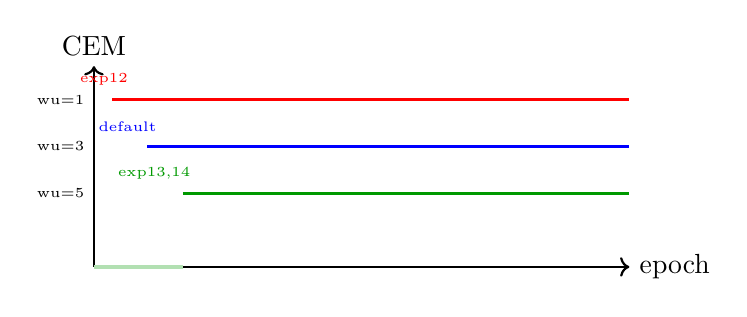
\begin{tikzpicture}[scale=0.85]
\draw[thick, ->] (0,0) -- (8,0) node[right] {epoch};
\draw[thick, ->] (0,0) -- (0,3) node[above] {CEM};

% warmup=1
\draw[very thick, red!30] (0,0) -- (0.27,0);
\draw[very thick, red] (0.27,2.5) -- (8,2.5);
\node[left, font=\tiny] at (0,2.5) {wu=1};

% warmup=3
\draw[very thick, blue!30] (0,0) -- (0.8,0);
\draw[very thick, blue] (0.8,1.8) -- (8,1.8);
\node[left, font=\tiny] at (0,1.8) {wu=3};

% warmup=5
\draw[very thick, green!60!black!30] (0,0) -- (1.33,0);
\draw[very thick, green!60!black] (1.33,1.1) -- (8,1.1);
\node[left, font=\tiny] at (0,1.1) {wu=5};

% labels
\node[font=\tiny, red] at (0.15, 2.8) {exp12};
\node[font=\tiny, blue] at (0.5, 2.1) {default};
\node[font=\tiny, green!60!black] at (0.9, 1.4) {exp13,14};
\end{tikzpicture}

\vspace{0.2cm}
\normalsize
Stages 3--6 are \textbf{completely skipped} during warmup.\\
$\Rightarrow$ Pure classification for first \param{warmup} epochs.

\end{column}
\begin{column}{0.48\textwidth}
\textbf{\param{epochs}: CosineAnnealing \& CEM full-power}

\vspace{0.2cm}
\small
Adaptive scaling: CEM is \warn{suppressed} when $lr > 0.00041$ (early training).

CEM reaches \good{full power} only in the final $\sim$5\% of epochs:

\vspace{0.2cm}
\begin{tabular}{ccc}
\toprule
\param{epochs} & Full-power & Extra \\
\midrule
240 (baseline) & $\sim$12 ep & --- \\
\textbf{300} & $\sim$15 ep & +25\% \\
\textbf{360} (exp19) & $\sim$18 ep & +50\% \\
\bottomrule
\end{tabular}

\vspace{0.3cm}
\normalsize
\textbf{exp19} uses 360 epochs specifically to extend the CEM full-power training window.
\end{column}
\end{columns}

\end{frame}

% ============================================================================
\begin{frame}{Experiment Groups: Design Rationale}

\begin{center}
\small
\begin{tabular}{clp{5.5cm}c}
\toprule
\textbf{Group} & \textbf{Experiments} & \textbf{Research Question} & \textbf{Stages Tested} \\
\midrule
\rowcolor{blue!5}
A & exp01--03 & Does increasing \param{lambd} \& \param{loss\_scale} alone improve defense? & 6, 8 \\
\rowcolor{teal!5}
B & exp04--07 & Can higher \param{noise} + stricter \param{var\_threshold} synergize? & 2, 6 \\
\rowcolor{violet!5}
C & exp08--11 & How do \param{slots} and \param{iters} affect clustering quality? & 3 \\
\rowcolor{orange!5}
D & exp12--14 & When should CEM activate? (\param{warmup} sensitivity) & 3--6 gate \\
\rowcolor{red!5}
E & exp15--18 & Do multi-dimensional improvements compound? & 2, 3, 4, 6, 8 \\
\rowcolor{green!5}
F & exp19--20 & Best candidates to beat SOTA & All \\
\bottomrule
\end{tabular}
\end{center}

\vspace{0.3cm}
\textbf{Strategy}: Groups A--D isolate individual factors via \textbf{controlled experiments}.\\
Groups E--F combine the best configurations from A--D to find optimal combinations.

\end{frame}

% ============================================================================
\begin{frame}{Group A (exp01--03): CEM Gradient Strength Sweep}

\textbf{Question}: Baseline effective strength = 8.0 is too weak. What happens if we push to 24--38?

\vspace{0.2cm}
\begin{center}
\small
\begin{tabular}{lccccccc}
\toprule
& \param{lambd} & \param{ls} & \textbf{Eff. Str.} & \param{noise} & \param{vt} & \param{slots} & \param{iters} \\
\midrule
\rowcolor{lightgray}
Baseline & 16 & 0.5 & \warn{8.0} & 0.05 & 0.15 & 8 & 3 \\
exp01 & \textbf{24} & \textbf{1.0} & \good{24.0} & 0.05 & 0.15 & 8 & 3 \\
exp02 & \textbf{32} & \textbf{1.0} & \good{32.0} & 0.05 & 0.15 & 8 & 3 \\
exp03 & \textbf{48} & \textbf{0.8} & \good{38.4} & 0.05 & 0.15 & 8 & 3 \\
\bottomrule
\end{tabular}
\end{center}

\vspace{0.2cm}
\begin{itemize}
    \item \textbf{Only Stages 6 \& 8 are changed}. All other stages identical to baseline.
    \item exp03 uses \param{ls}=0.8 (not 1.0) because $48 \times 1.0 = 48$ might be too aggressive and crash classification accuracy.
    \item \textbf{Expected}: monotonic SSIM decrease (better privacy) with possible accuracy trade-off at exp03.
\end{itemize}

\end{frame}

% ============================================================================
\begin{frame}{Group B (exp04--07): Noise + Threshold Push}

\textbf{Question}: Can we improve defense by pushing \param{noise} (Stage 2) and \param{var\_threshold} (Stage 6) simultaneously?

\vspace{0.2cm}
\begin{center}
\small
\begin{tabular}{lcccccc}
\toprule
& \param{lambd} & \param{noise} & \param{vt} & \param{ls} & \textbf{Eff. Str.} & \textbf{Threshold} \\
\midrule
\rowcolor{lightgray}
Baseline & 16 & 0.05 & 0.15 & 0.5 & 8.0 & 3.75e-4 \\
exp04 & 24 & \textbf{0.08} & \textbf{0.20} & 1.0 & 24.0 & \textbf{1.28e-3} \\
exp05 & 32 & \textbf{0.08} & \textbf{0.20} & 0.8 & 25.6 & \textbf{1.28e-3} \\
exp06 & 24 & \textbf{0.06} & \textbf{0.25} & 1.0 & 24.0 & \textbf{9.00e-4} \\
exp07 & 32 & \textbf{0.10} & \textbf{0.20} & 0.8 & 25.6 & \textbf{2.00e-3} \\
\bottomrule
\end{tabular}
\end{center}

\vspace{0.2cm}
\begin{itemize}
    \item \textbf{exp06}: minimal noise increase (0.05$\to$0.06) but maximum \param{vt} (0.25) --- tests ``strict threshold, low noise'' strategy
    \item \textbf{exp07}: extreme noise (0.10 = 2$\times$ baseline) --- tests privacy at the cost of classification accuracy
    \item Threshold increases 2.4$\times$ to 5.3$\times$ vs baseline
\end{itemize}

\end{frame}

% ============================================================================
\begin{frame}{Group C (exp08--11): Slot Attention Architecture Search}

\textbf{Question}: How do \param{slots} and \param{iters} affect clustering quality? (Controlled experiment: only Stage 3 changes)

\vspace{0.2cm}
\begin{center}
\small
\begin{tabular}{lccccl}
\toprule
& \param{slots} & \param{iters} & \param{heads} & \textbf{Eff. Str.} & \textbf{What Changed} \\
\midrule
\rowcolor{lightgray}
Baseline & 8 & 3 & 4 & 8.0 & --- \\
exp08 & \textbf{16} & 3 & 4 & 24.0 & $2\times$ prototypes \\
exp09 & \textbf{4} & 3 & 4 & 24.0 & $0.5\times$ prototypes \\
exp10 & 8 & \textbf{5} & 4 & 32.0 & +2 GRU iterations \\
exp11 & \textbf{12} & \textbf{4} & 4 & 24.0 & Balanced middle \\
\bottomrule
\end{tabular}
\end{center}

\vspace{0.3cm}
\begin{columns}[T]
\begin{column}{0.48\textwidth}
\textbf{Slots trade-off:}
\begin{itemize}
    \item Too few (4): coarse clustering, 530 classes mapped to 4 prototypes
    \item Too many (16): slot collapse risk (some slots ``die'' and never get assigned features)
\end{itemize}
\end{column}
\begin{column}{0.48\textwidth}
\textbf{Iterations trade-off:}
\begin{itemize}
    \item 3 iterations: may not fully converge slot competition
    \item 5 iterations: more refined, but +67\% compute and potential vanishing gradients
\end{itemize}
\end{column}
\end{columns}

\end{frame}

% ============================================================================
\begin{frame}{Group D (exp12--14): Warmup Sensitivity}

\textbf{Question}: How much does the CEM activation timing matter?

\vspace{0.2cm}
\begin{center}
\small
\begin{tabular}{lcccccl}
\toprule
& \param{wu} & \param{lambd} & \param{noise} & \param{vt} & \param{ls} & \textbf{Strategy} \\
\midrule
\rowcolor{lightgray}
Baseline & 3 & 16 & 0.05 & 0.15 & 0.5 & Default \\
exp12 & \textbf{1} & 24 & 0.07 & 0.20 & 1.0 & Aggressive: CEM from epoch 2 \\
exp13 & \textbf{5} & 32 & 0.06 & 0.20 & 1.0 & Conservative: classifier first \\
exp14 & \textbf{5} & 24 & 0.07 & 0.20 & \textbf{1.2} & Late start, compensate with $\uparrow$ls \\
\bottomrule
\end{tabular}
\end{center}

\vspace{0.3cm}
\begin{columns}[T]
\begin{column}{0.48\textwidth}
\textbf{warmup=1 (exp12):}
\begin{itemize}
    \item CEM starts when accuracy $<5\%$
    \item Risk: encoder learns to scatter features before learning to classify
    \item Possible benefit: features never ``crystallize'' into attack-friendly patterns
\end{itemize}
\end{column}
\begin{column}{0.48\textwidth}
\textbf{warmup=5 + ls=1.2 (exp14):}
\begin{itemize}
    \item Classifier converges for 5 epochs first
    \item CEM ``late arrival'' compensated by 20\% amplified loss scale
    \item Effective strength: $24 \times 1.2 = 28.8$
\end{itemize}
\end{column}
\end{columns}

\end{frame}

% ============================================================================
\begin{frame}{Groups E \& F: Combined Configs and Best Candidates}

\small
\textbf{E (exp15--18)}: Multi-dimensional improvements \quad \textbf{F (exp19--20)}: Final candidates

\vspace{0.1cm}
\begin{center}
\adjustbox{max width=\textwidth}{
\scriptsize
\begin{tabular}{lcccccccccc}
\toprule
& \param{$\lambda$} & \param{$\sigma$} & \param{vt} & \param{ls} & \param{sl} & \param{hd} & \param{it} & \param{wu} & \param{ep} & \textbf{Eff.} \\
\midrule
\rowcolor{lightgray}
Baseline & 16 & .05 & .15 & 0.5 & 8 & 4 & 3 & 3 & 240 & 8.0 \\
\midrule
exp15 & \textbf{40} & .06 & .20 & 1.0 & \textbf{12} & 4 & \textbf{4} & 3 & 300 & \good{40.0} \\
exp16 & 36 & .07 & \textbf{.25} & 0.8 & 8 & 4 & \textbf{4} & \textbf{5} & 300 & 28.8 \\
exp17 & \textbf{48} & \textbf{.08} & \textbf{.25} & 0.8 & 8 & 4 & 3 & \textbf{5} & 300 & \good{38.4} \\
exp18 & 28 & .07 & .20 & 1.0 & \textbf{10} & \textbf{2} & \textbf{4} & 3 & 300 & 28.0 \\
\midrule
exp19 & \textbf{40} & .06 & .20 & 1.0 & 8 & 4 & \textbf{5} & 3 & \textbf{360} & \good{40.0} \\
exp20 & 36 & .06 & \textbf{.25} & \textbf{1.2} & \textbf{12} & 4 & \textbf{4} & \textbf{5} & 300 & \good{\textbf{43.2}} \\
\bottomrule
\end{tabular}
}
\end{center}

\vspace{0.1cm}
\begin{itemize}
    \small
    \item \textbf{exp19}: 360 epochs $\Rightarrow$ 18 epochs full-power CEM (vs 12 baseline)
    \item \textbf{exp20}: highest eff.\ strength (43.2 = $5.4\times$ baseline), strictest threshold, most slots
\end{itemize}

\end{frame}

% ============================================================================
\begin{frame}{Summary: Parameter $\leftrightarrow$ Stage Mapping}

\begin{center}
\scriptsize
\begin{tabular}{p{1.8cm}cp{3.5cm}p{3cm}p{2.5cm}}
\toprule
\textbf{Parameter} & \textbf{Stage} & \textbf{What It Controls} & \textbf{$\uparrow$ Benefit} & \textbf{$\uparrow$ Risk} \\
\midrule
\param{noise} ($\sigma$) & 2, 6 & Noise std + CEM threshold & Harder reconstruction & Lower accuracy \\
\param{slots} & 3 & \# soft-cluster prototypes & Finer clustering & Slot collapse \\
\param{iters} & 3 & GRU refinement rounds & Better convergence & Computation cost \\
\param{heads} & 4 & Multi-head perspectives & More diverse views & Narrow head dims \\
\param{var\_thr} & 6 & Variance strictness & Stronger dispersion & Training instability \\
\param{loss\_scale} & 6$\to$8 & CEM loss amplifier & Stronger CEM signal & Accuracy loss \\
\param{lambd} & 8 & Gradient injection coeff. & Stronger encoder push & CE grad drowned \\
\param{warmup} & 3--6 & CEM activation delay & Stable classification & Less defense time \\
\param{epochs} & all & Training duration & Longer full-power CEM & Wall-clock time \\
\bottomrule
\end{tabular}
\end{center}

\vspace{0.3cm}
\begin{block}{Success Criterion}
Find a configuration where \textbf{Inference SSIM $<$ 0.532} while maintaining reasonable classification accuracy ($>$60\%). Results pending.
\end{block}

\end{frame}

% ============================================================================
\begin{frame}{}
\vfill
\begin{center}
{\Huge\textbf{Thank You}}

\vspace{1cm}
{\large Experiments are currently running on the server.\\
Results will be available in \texttt{run3log\_*/summary.csv}}

\vspace{0.8cm}
{\normalsize 20 experiments $\times$ $\sim$5h each $\approx$ 100 hours total}
\end{center}
\vfill
\end{frame}

\end{document}
